 \documentclass[10.5pt,twocolumn]{jbuaa}


%%画圆圈数字
\newcommand*\circled[1]{\tikz[baseline=(char.base)]{
            \node[shape=circle,draw,inner sep=1pt] (char) {#1};}}
            
%取消英文连词符
% \tolerance=1
% \emergencystretch=\maxdimen
% \hyphenpenalty=10000
% \hbadness=10000

\newcommand\mycolorRed[1]{{\color{red}#1}}
\newcommand\mycolorYellow[1]{{\color{yellow}#1}}
% \newcommand*\mycolorRed{\color{red}}

%%%????? 公式中字体的定义尺寸为 10 磅,上标/下标 68%,次下标/上标 42% ?????? 
\DeclareMathSizes{10.5}{10}{6.8}{4.2}
%%%% 本示例中带单位的数据采用的是siunitx来生成,好像默认与公式同样大小的字体,所以数字在正文中会小一些
%%%% 行文中普通数字大小为10.5pt,公式里或者用siunitx生成的数字则会是10pt,多少有点不协调。

%%%设置公式前后距离,差不多近似
\setlength{\abovedisplayskip}{2.5mm}
\setlength{\belowdisplayskip}{2.5mm}


\usepackage{tabu}
\usepackage{longtable}
\usepackage{makecell}
\renewcommand\cellgape{\Gape[-3pt][-3pt]}


%%%%%%%%%%%%%%%%%%%%%%%%%%%%%%%%%%%%%%%%%%%%%%%%%%%%%%%%%%%%%%%%
%      文章正文
%%%%%%%%%%%%%%%%%%%%%%%%%%%%%%%%%%%%%%%%%%%%%%%%%%%%%%%%%%%%%%%%
\begin{document}
%%%%%%%%%%%%%%%%%%%%%%%%%%%%%%%%%%%%%%%%%%%%%%%%%%%%%%%%%%%%%%%%
% 标题,基金项目,作者,通信地址定义
%%%%%%%%%%%%%%%%%%%%%%%%%%%%%%%%%%%%%%%%%%%%%%%%%%%%%%%%%%%%%%%%
\title{
% \vspace{1cm} \erhao\hei 这个是标题,这个是标题,这个是标题 \vspace{-0.2cm}
\erhao\hei Dependency-aware and Predictive Microservices Auto-Scaling in Cost-effective Platform-as-a-Service Clouds \vspace{-0.2cm}
}

\author{
% \sihao\fang 彭青蓝 \\[0.1cm]
\sihao\fang 彭青蓝 \makebox{$^{\text{1}}$}\\[0.1cm]
\liuhao (1.~~浙江大学~~软件学院,宁波~~315000)\\ 
}

\date{}  

\CKeyword{微服务; 自动扩容; 多元时间序列预测; 相空间重构; RBF神经网络}
\PaperNo{001}

\twocolumn[
  \begin{@twocolumnfalse}
  \maketitle
\begin{CAbstractJBUAA}
为了更好地把握微服务架构中各个服务的负载趋势,以便做出及时准确的微服务伸缩策略,提出了一种基于多元时间序列的负载预测方法。充分考虑到具有相互依赖的微服务之间负载存在关联,采用相空间重构将多个具有依赖关系的微服务的负载历史数据映射到一个动力系统中,近似地恢复多个微服务之间的多维非线性关系。使用RBF神经网络预测模型,实现微服务负载的动态多部预测,并根据预测负载生成微服务实例伸缩策略。
\end{CAbstractJBUAA}
%%%%%%%%首页角注
\positiontextbox{2.0cm}{25cm}{
\noindent\rule{4cm}{.5pt}\\[0.5ex]%
\hspace*{1em} \liuhao \linespread{0.8}\selectfont
\parbox{\textwidth}{%
\hei\makebox[\widthof{\makebox{*}}][r]{起}草日期: 2018-02-11\\%
\hei\makebox[\widthof{\makebox{*}}][r]{修}改日期: 2018-02-11\\%
}}
  \end{@twocolumnfalse}
]


%%%%%%%%%%%%%%%%%%%%%%%%%%%%%%%%%%%%%%%%%%%%%%%%%%%%%%%%%%%%%%%%
%  正文由此开始-------------------------
%%%%%%%%%%%%%%%%%%%%%%%%%%%%%%%%%%%%%%%%%%%%%%%%%%%%%%%%%%%%%%%%
%%%%%%%%%%%%%%%%%%%%%%%%%%%%%%%%%%%%%%%%%%%%%%%%%%%%%%%%%%%%%%%%
\wuhao 
%  分栏开始


\section{从单体式架构到微服务架构}
传统的单体式应用存在应用内部结构复杂、人员协调困难、可靠性低的问题。随着信息技术的飞速发展,互联网企业又面临着新的挑战:1)用户规模大,对分布式要求高;2)迭代周期短,每天都要发布多个新版本;3)技术迭代快,不同团队采用的技术不同。

幸运的是,敏捷开发方法创始人之一,ThoughtWorks首席科学家Martin Fowler与2014年提出了微服务式架构,恰逢容器技术发展元年,随着容器技术的飞速发展,微服务架构逐渐落地生根。国外的包括Netflix,Amazon和eBay在内的大多数大型网站已经从单一的体系结构演变为微服务体系结构。国内的知乎、豆瓣已经完全演化为微服务架构,阿里、京东也进行了一些微服务实践。

图1(a)是一个电商平台的单体式架构,尽管采用了模块化逻辑,但是最终还是会被打包并部署为单体式应用。

\begin{figure}[H]
\centering
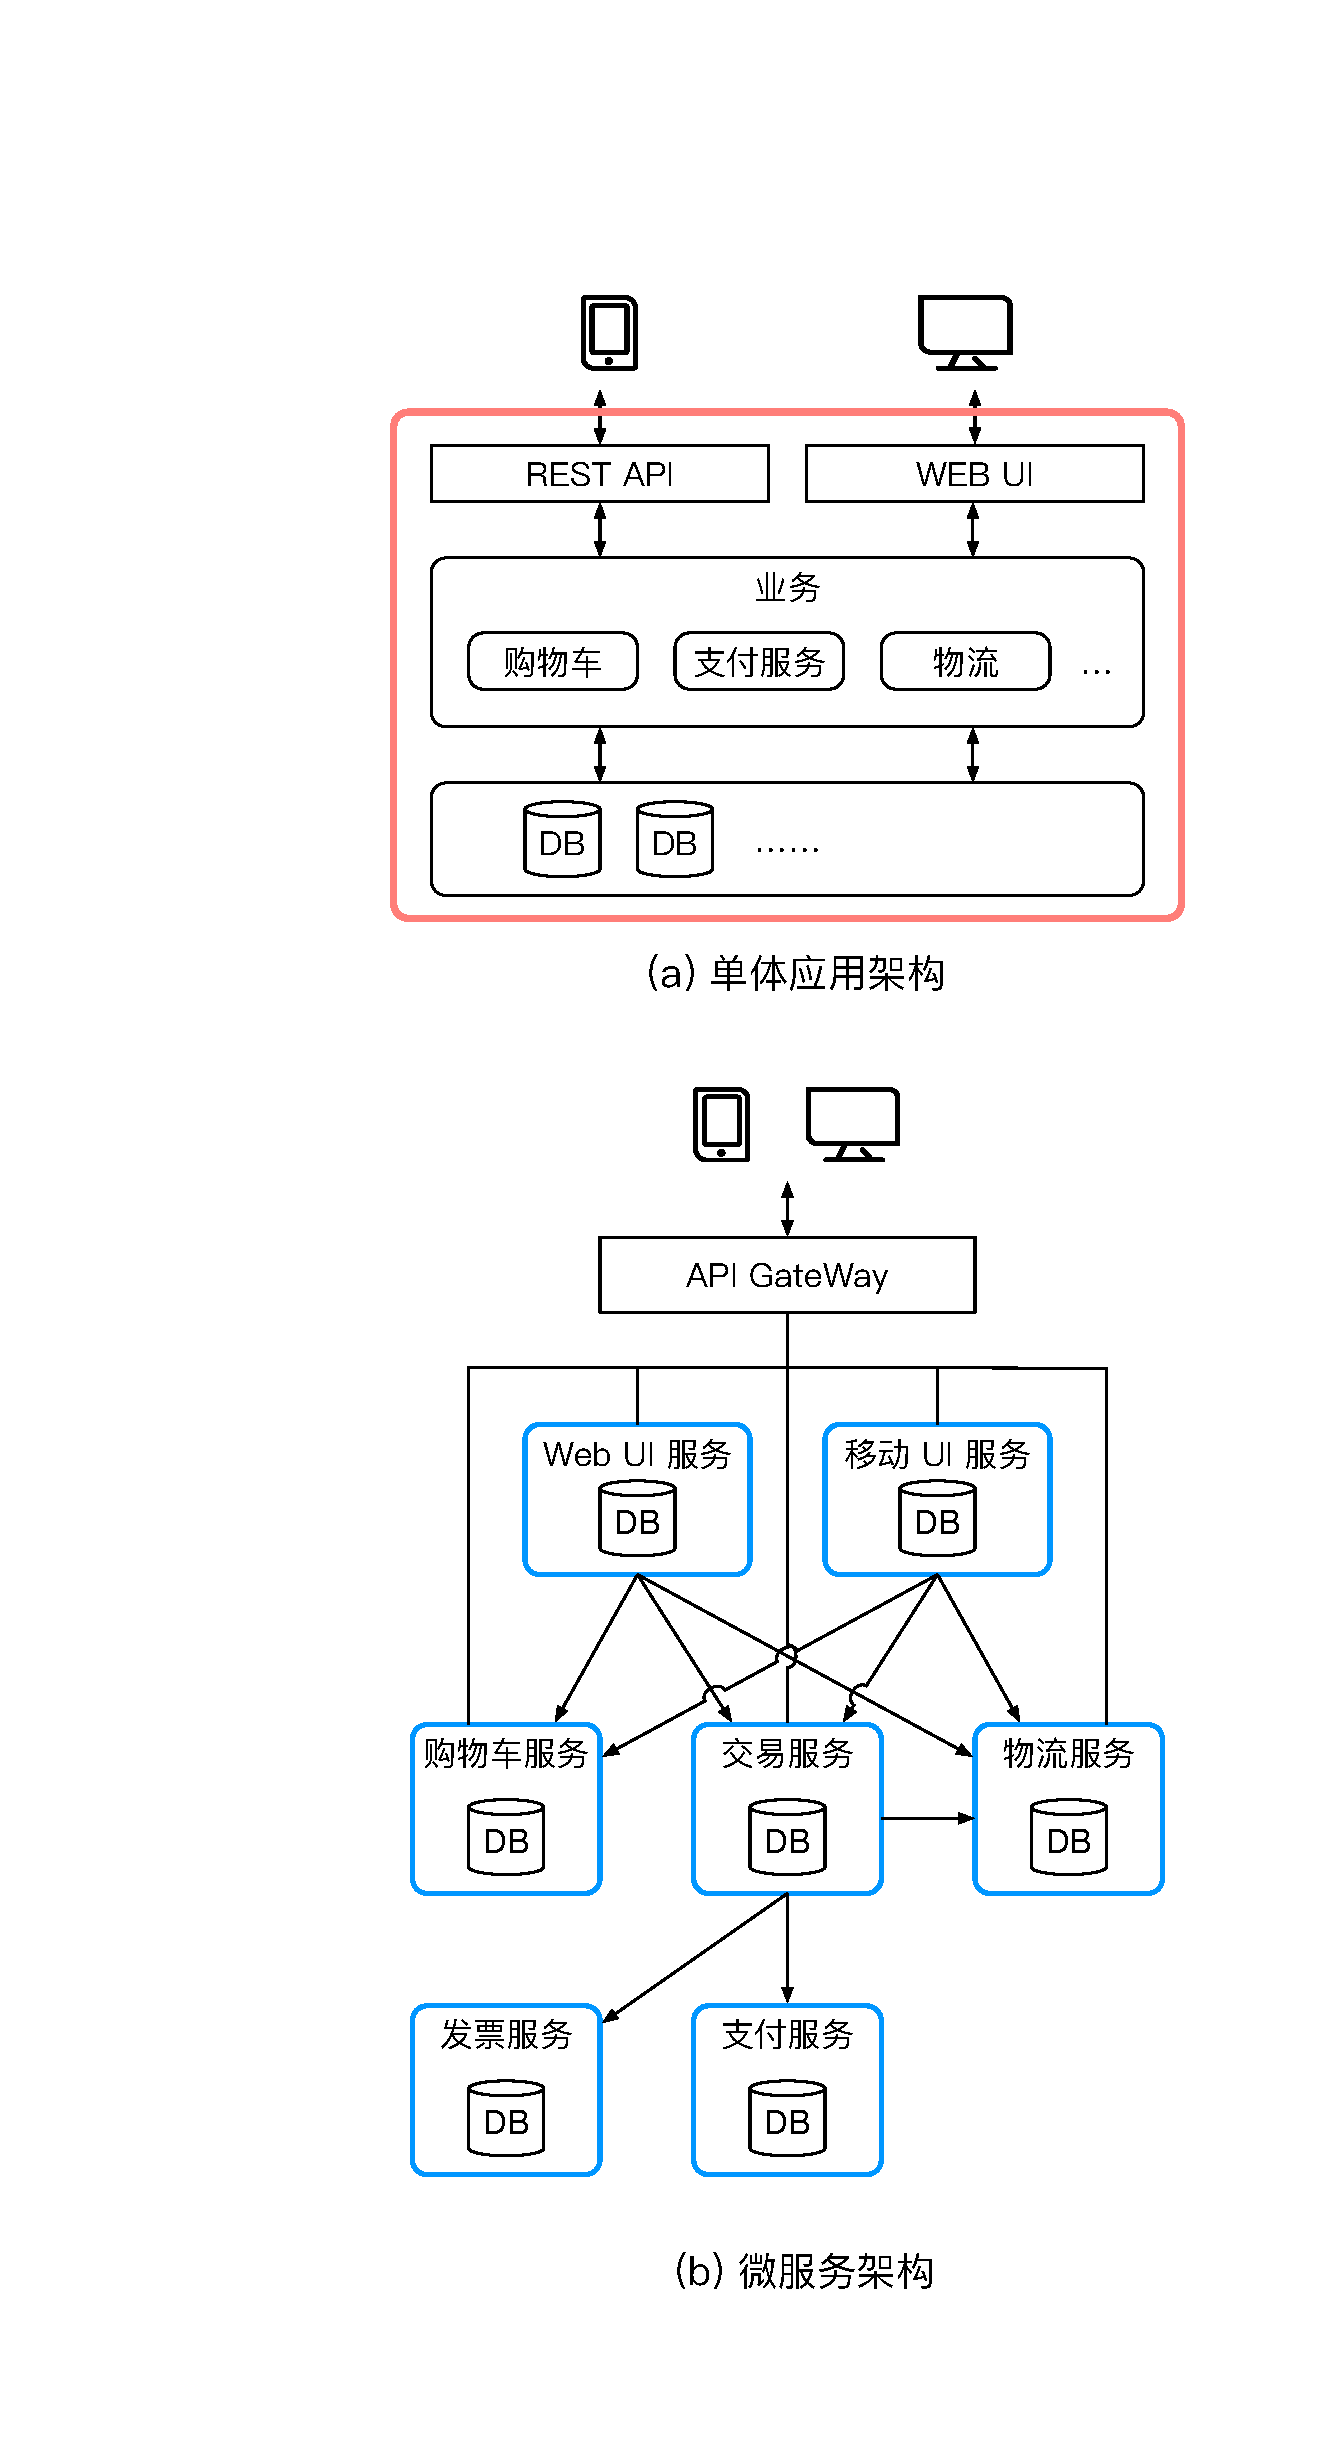
\includegraphics [scale=0.4,trim=0 0 0 0]{./image/1.pdf}
\caption{一个电商平台的不同架构}
\end{figure}

同样的案例采用微服务式架构,如图1(b)所示,对于每一个应用功能点都使用微服务完成。不像传统多个服务共享一个数据库(这里指SOA架构),微服务架构每个服务都有自己的数据库。

% 微服务架构带来的优点:

% 1)巨大单体式应用被分解为多个微服务,通过REST API互相沟通,解决了复杂性问题。单个服务很容易开发、理解和维护。

% 2)使得每个服务都可以有专门开发团队来开发。开发者可以自由选择开发技术,提供API服务。

% 3)每个微服务独立的部署,开发者不再需要协调其它服务部署对本服务的影响,使得持续化部署成为可能。(不用联调)

% 4)每个服务可以独立扩展。

\section{微服务架构的自动伸缩}
\subsection{服务可以独立伸缩}
微服务架构在带来一个好处是每个服务可以独立地进行扩展,做到有针对性的扩容。
\begin{figure}[H]
\centering
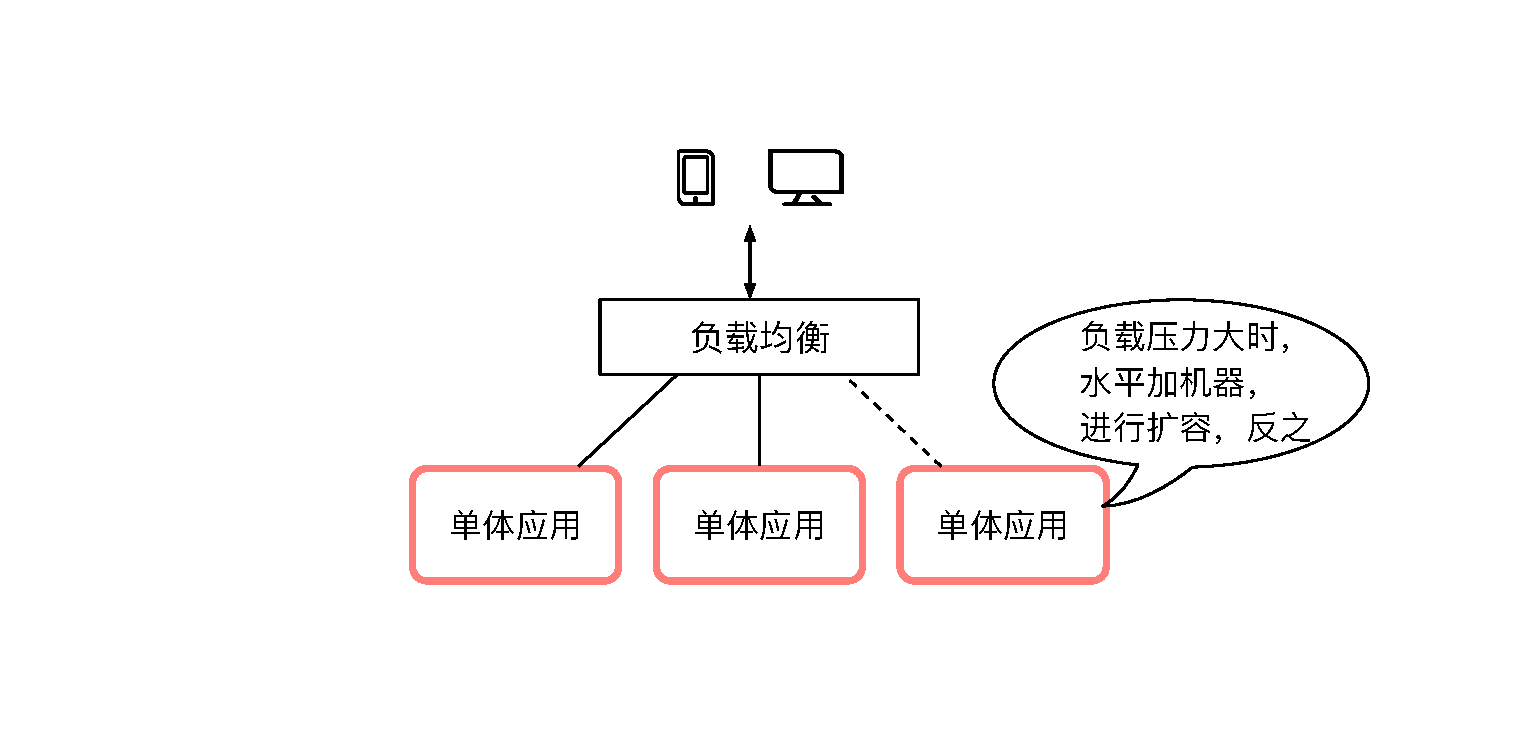
\includegraphics [scale=0.4,trim=0 0 0 0]{./image/2.pdf}
\caption{单体式架构的伸缩}
\end{figure}

例如针对双十一零时的用户高峰,图2是一个传统的单体式应用的扩容方案,采用了增加电商单体应用实例的方式来应对即将到来的高峰。
\begin{figure}[H]
\centering
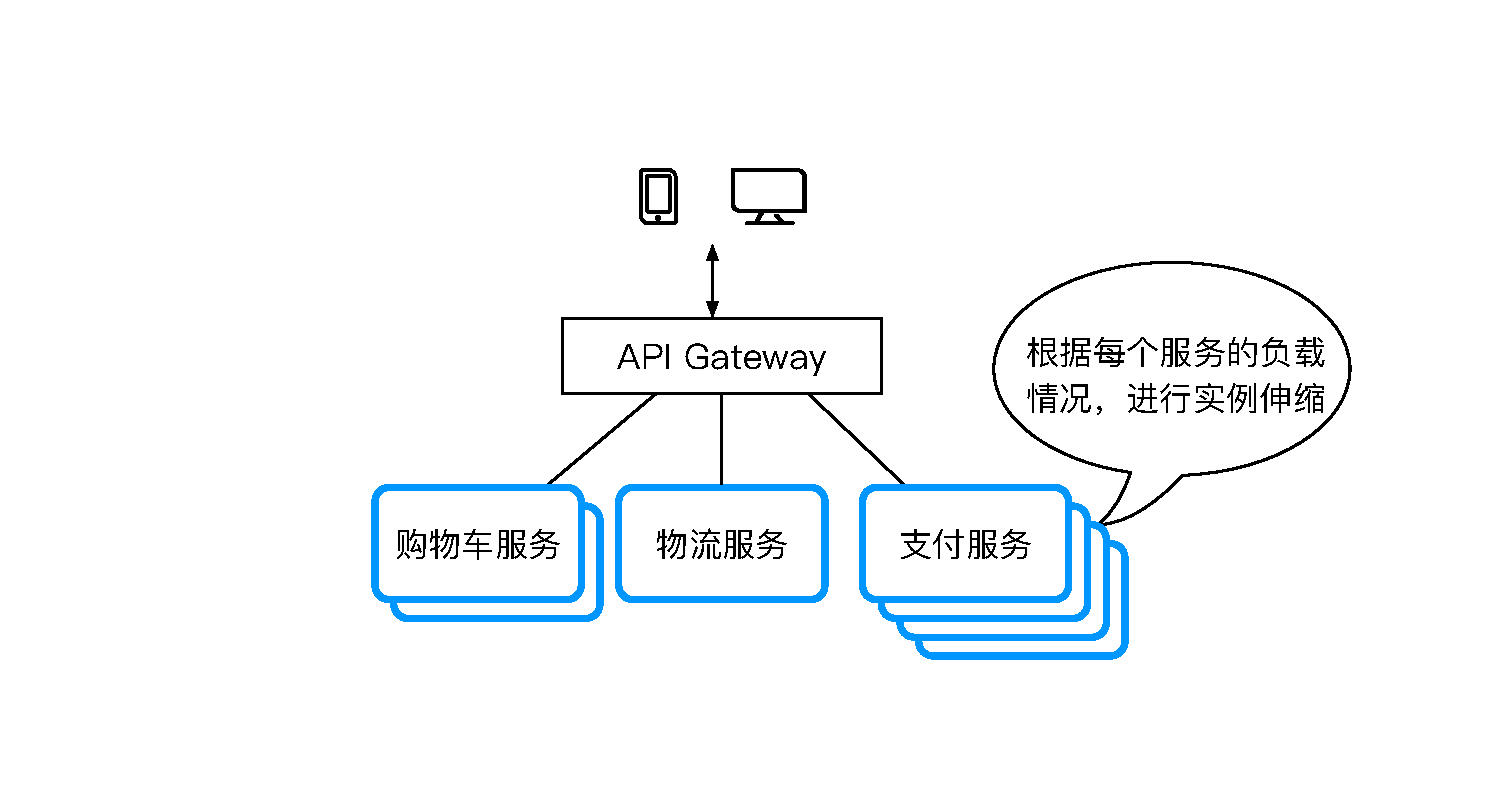
\includegraphics [scale=0.4,trim=0 0 0 0]{./image/3.pdf}
\caption{微服务架构的伸缩}
\end{figure}

图3是微服务架构的扩容方案。由于大家提前都将商品加入购物车中了,因此购物车服务在零点压力不太大,压力主要集中在支付服务。采用微服务架构后,就可以单独添加支付服务的实例来应对高峰,从而做到了有针对性的扩容,节省了计算资源。

\begin{figure*}[!t]
\centering
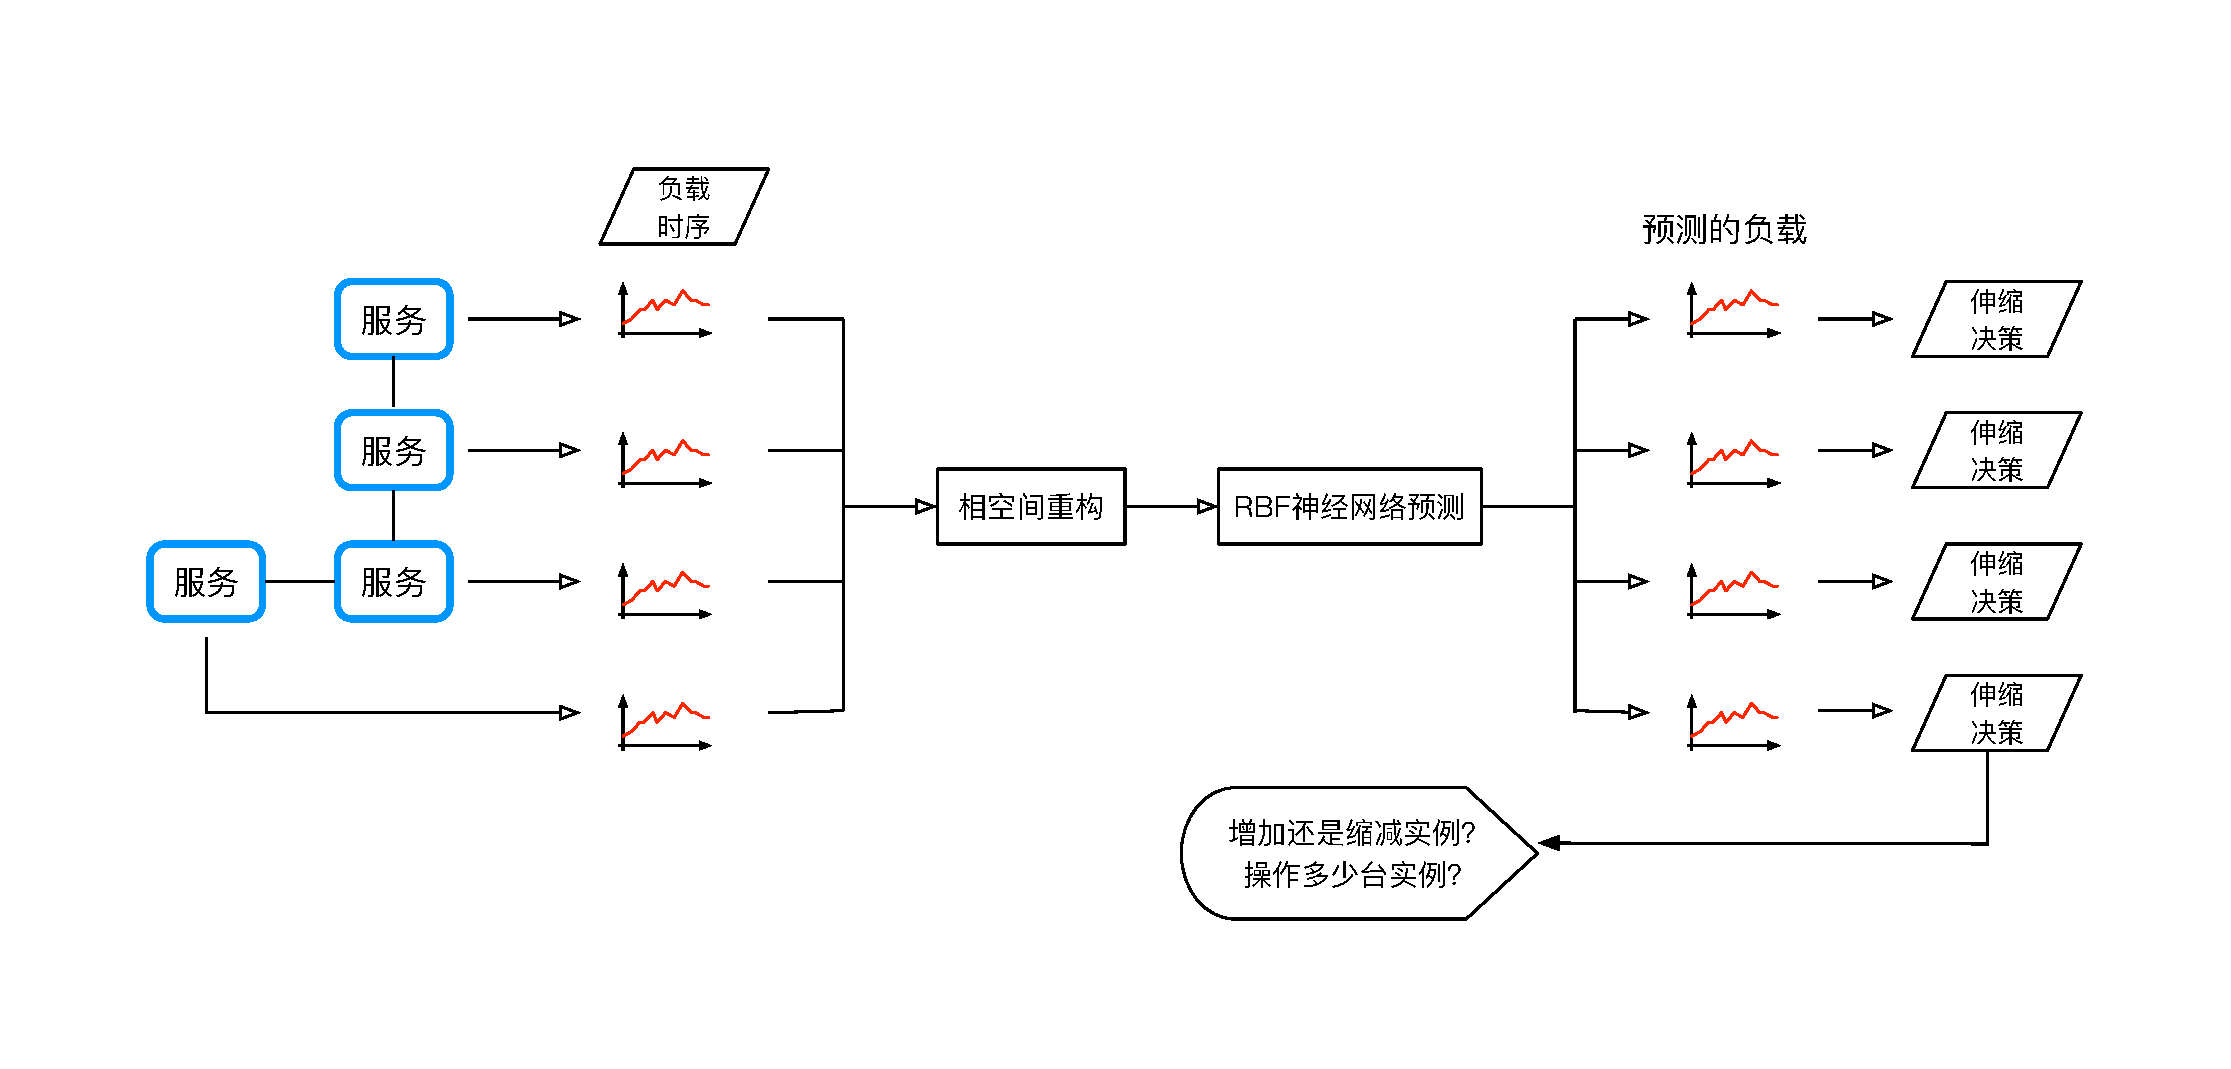
\includegraphics [scale=0.5,trim=0 0 0 0]{./image/7.pdf}
\caption{基于服务依赖感知和预测的自动伸缩机制}
\end{figure*}

\subsection{服务之间存在依赖关系}
采用微服务架构后,各个服务之间存在依赖关系。
\begin{figure}[H]
\centering
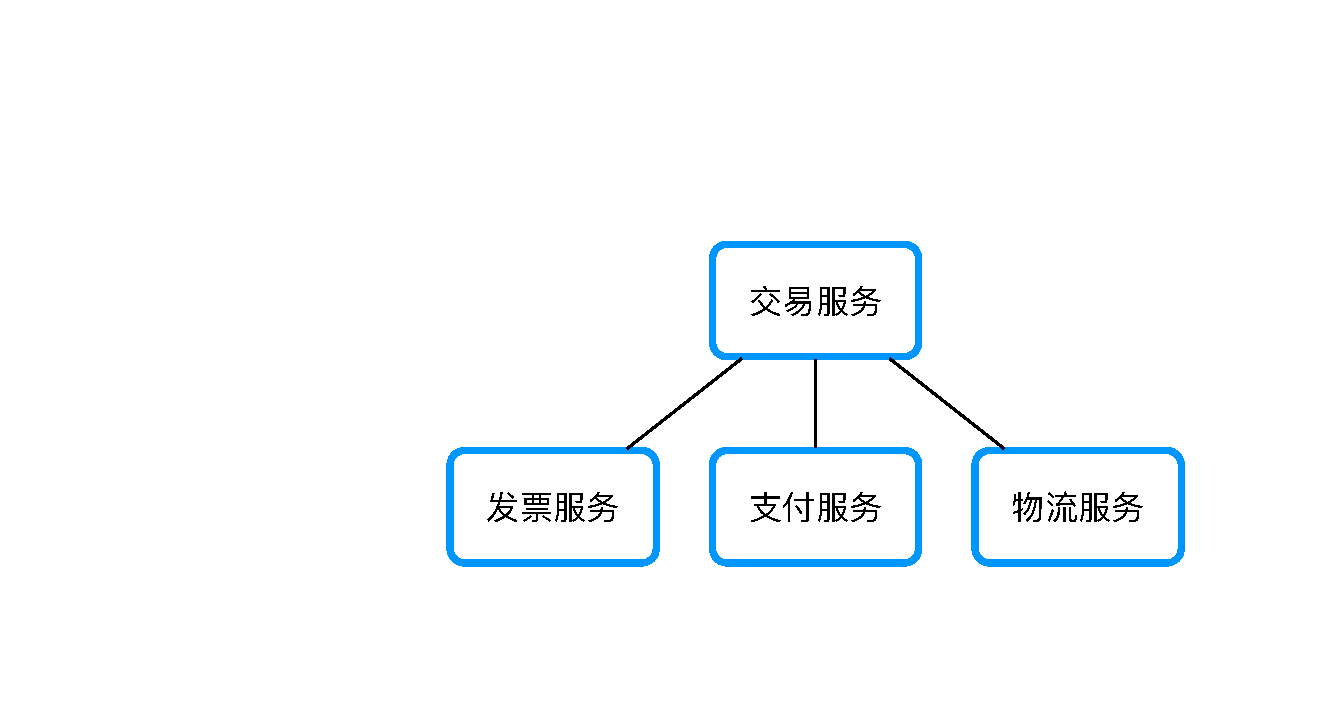
\includegraphics [scale=0.4,trim=0 0 0 0]{./image/4.pdf}
\caption{服务之间的依赖}
\end{figure}
如图4所示交易服务需要按照顺序调用发票服务、支付服务与物流服务,因此支付服务于这三个服务之间存在依赖关系。所以交易服务的负载变化明显会影响到发票、支付与物流服务的负载变化。反过来,当发票服务由于内部设计的缺陷或者是某种不确定因素导致负载上升时,这种变化也会影响到上层依赖它的交易服务。因此各个服务负载间的相互影响是存在的,并且呈现出一种非线性、动态多变的特点。服务实例的伸缩不能仅考虑当前服务的负载,应当将个依赖链的相互影响考虑在内。

\section{基于服务依赖感知和预测的自动伸缩机制}
该机制首先找出将微服务架构中的动力系统,然后使用张鹏程等人在\cite{Service2018}中提出的多元时间序列方法预测各个服务未来的负载,并根据该预测值作出相应的伸缩策略。
\subsection{动力系统的划分}
\begin{figure}[H]
\centering
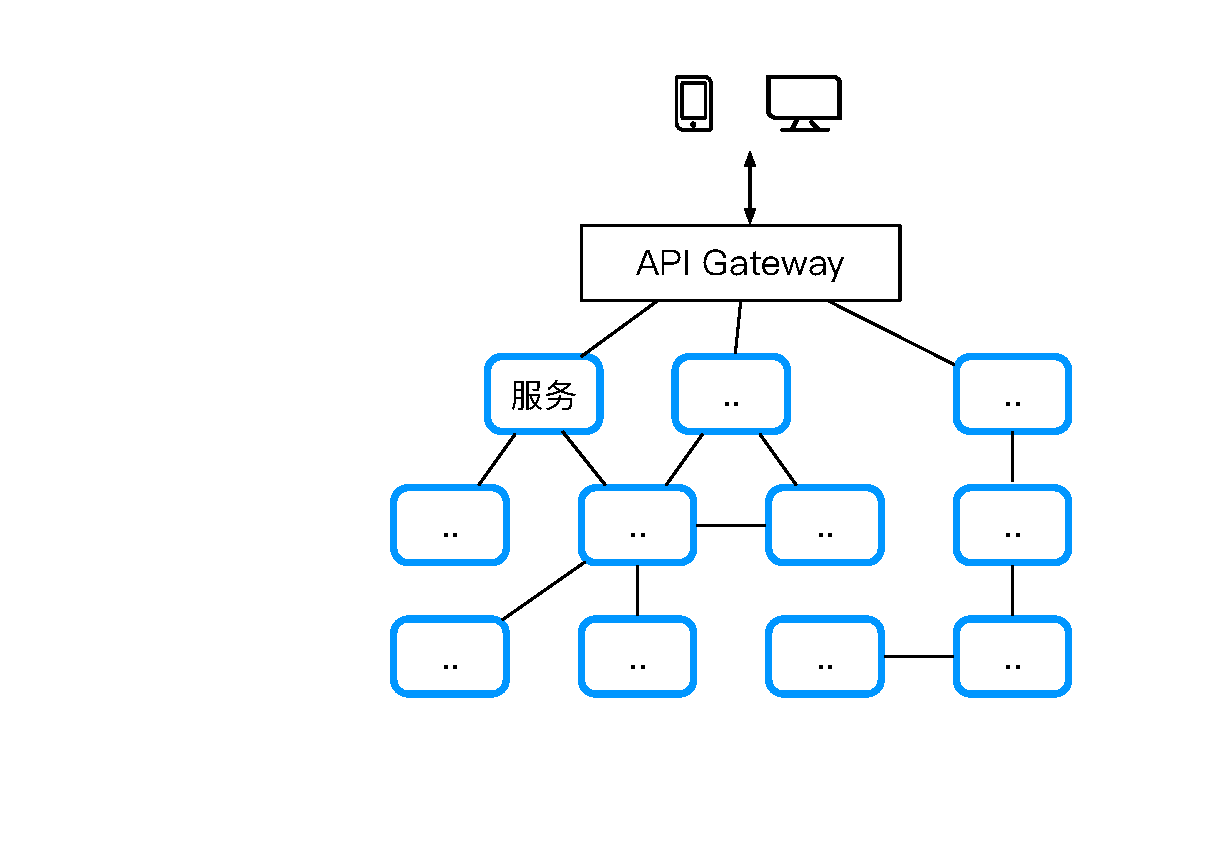
\includegraphics [scale=0.4,trim=0 0 0 0]{./image/5.pdf}
\caption{服务之间的拓扑结构}
\end{figure}
如图5所示,一个应用的微服务架构可以用一个图$T=(V,E)$来表示,其中$V=\{S_1,S_2,S_3,......S_n\}, V=\{e_{i,j}...\}$。图中每个顶点表示一个独立的服务,它可以拥有多个实例,这些事例根据该服务的负载动态伸缩。边$e_{i,j}$表示服务$S_i$和服务$S_j$之间存在依赖。图$T$可以从微服务架构中的注册中心获得。
\begin{figure}[H]
\centering
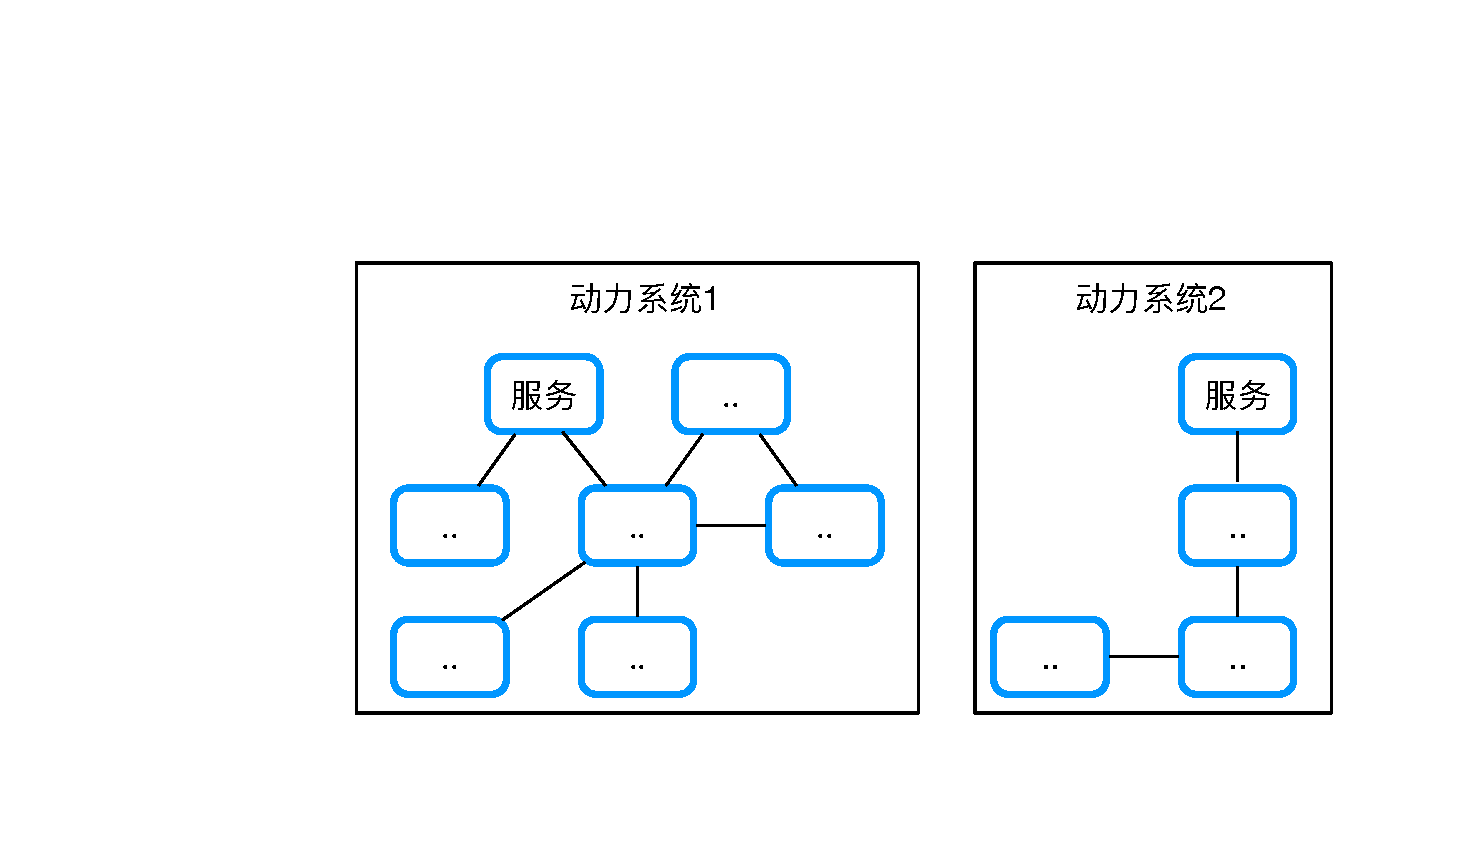
\includegraphics [scale=0.4,trim=0 0 0 0]{./image/6.pdf}
\caption{动力系统的划分}
\end{figure}
如图6所示,首先找出该图中的所有联通分量,每个联通分量中的服务之间存在着依赖关系。可以将每个联通分量看做一个独立的动力系统,每个动力系统中的元素之间以一种混沌的方式互相影响。



\subsection{相空间重构}
非线性时间序列可以看作由确定的非线性系统产生的,相空间(Phase space)是描述系统运动和演变最有力 的工具之一,可以表示动力系统中所有可能的状态,其中每个状态具有对应的相位空间点,从而刻画了一个点随时间变化的情况。
在得到一个动力系统中所有服务的负载时间序列后,就可以使用相空间重构来近似恢复序列构成的动力系统。

\subsection{RBF神经网络}
RBF神经网络由Moody和Darken根据人体大脑皮层的感知区域特点提出的一种前馈型神经网络,将一个动力系统的负载综合数据序列作为输入进行预测。然后分解得到每个服务的负载预测值,根据预测值再作出伸缩决策。以图6中的动力系统2为例,整个伸缩过程如图7所示。



\section{实验设计}

\subsection{对比方法}
实验就以下三种扩容机制进行对比:

1)基于阈值触发的扩容机制

2)基于预测的扩容机制

3)基于服务依赖感知和预测的扩容机制

\subsection{数据集}

\subsection{实验步骤}

\subsection{预计结果}




%%%%%%%%%%%%%%%%%%%%%%%%%%%%%%%%%%%%%%%%%%%%%%%%%%%%%%%%%%%%%%%%
%  参考文献
%%%%%%%%%%%%%%%%%%%%%%%%%%%%%%%%%%%%%%%%%%%%%%%%%%%%%%%%%%%%%%%%

\renewcommand\refname{\hei\wuhao\centerline{参考文献}\global\def\refname{参考文献}}
\vskip 12pt

\let\OLDthebibliography\thebibliography
\renewcommand\thebibliography[1]{
  \OLDthebibliography{#1}
  \setlength{\parskip}{0pt}
  \setlength{\itemsep}{0pt plus 0.3ex}
}

{
\renewcommand{\baselinestretch}{0.9}
\liuhao
\bibliographystyle{unsrt}
\bibliography{./TempExample}
}



\end{document}
